\section{Dal tempo continuo al tempo discreto}
Per arrivare a parlare dei segnali a tempo discreto cominciamo a capire come si passa da un segnale a tempo continuo ad uno a tempo discreto.

\begin{figure}[ht!]
    \centering
    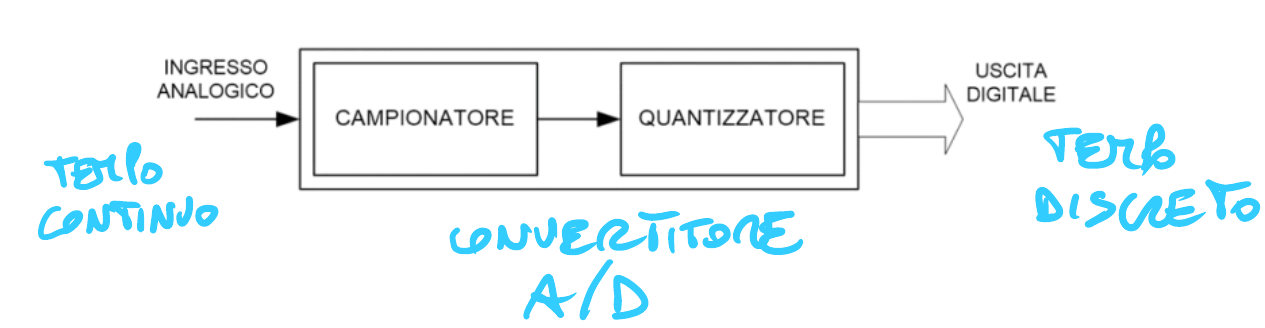
\includegraphics[scale=0.35]{immagini/lez9/convertitoreAD.jpg}
\end{figure}

Per fare questo passaggio si usa un convertitore A/D (analogico digitale) che prende in input un segnale a tempo continuo e ci fornisce in output un segnale a tempo discreto.

\subsection{Campionatore}
E' il componente del convertitore che fa il campionamento. Ho un segnale a tempo continuo e ne considero solo alcuni campioni, ad esempio se il nostro segnale e': $x(t) = A \cos{(2\pi f_0 t + \varphi_0)}$, si decide un intervallo di campionamento $T_c$ che e' in pratica la distanza tra due campioni. Di conseguenza sostituendo a t $n T_c$ si ottiene il segnale a tempo discreto:
\[
    x(\textcolor{red}{nTc}) = A \cos(2\pi f_0 \textcolor{red}{nTc} + \varphi_0)
\]

Il nostro obbiettivo sara' capire come campionare bene. Nella maggior parte dei casi campioneremo in modo uniforme, ovvero c'e' una distanza uguale tra un campione e l'altro, ma si puo' anche campionare in modo non uniforme.

\begin{figure}[ht!]
    \centering
    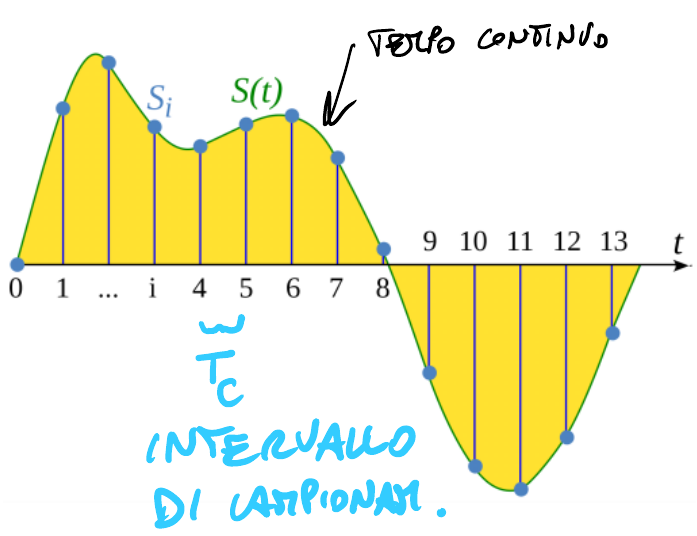
\includegraphics[scale=0.35]{immagini/lez9/campionatore.jpg}
\end{figure}

\subsection{Quantizzatore (quantizzazione)}
Possiamo considerarlo come una funzione matematica tale per cui in ingresso c'e' un segnale reale ed in uscita' c'e' un segnale che appartiene ad un sottoinsieme di numeri interi.

In pratica e' come se facessimo un arrotondamento di un decimale ad una certa posizione, facciamo un approssimazione del segnale scegliendo quanti campioni prendere.
Il least siginificant bit e' dato da : $\frac{\mbox{RANGE}}{2^{n_q}}$, dove il denominatore e' il numero di bit di quantizzazione.

\section{Osservazioni su segnali discreti}
Per fare un passo avanti per capire come campionare, analizziamo alcune caratteristiche di un segnale campionato, ovvero discreto.

Cominciamo dando della terminologia, diremo \underline{intervallo di campionamento} (espresso in secondi e costante) $T_s$ mentre diremo \underline{frequenza di campionamento} o sampling frequency $f_c = \frac{1}{T_c}$, espressa in Hz.

\subsection{La frequenza discreta e' adimensionale}
Se abbiamo un segnale tempo continuo e lo campioniamo, ricordando che $T_c = \frac{1}{f_c}$ otteniamo:
\[
    x[n] = x(n T_c) = A \cos{(2\pi f_0 \frac{n}{f_c} + \varphi_0)}
\]

Se consideriamo l'argomento del coseno in cui compare la frequenza:
\[
    \Tilde{\omega} = 2\pi \frac{f_0}{f_c}
\]

Lo chiameremo \textbf{velocita' angolare o pulsazione discreta} ed e' misurata in radianti (RAD).
Mentre se prendiamo la \textbf{frequenza discreta}:

\[
    \frac{f_0}{f_c} = \Tilde{f}
\]

e ne facciamo l'analisi dimensionale vediamo che sono Hz fratto Hz, quindi e' una grandezza adimensionale che \textbf{NON} ha niente a che vedere con il tempo.

\subsubsection{Corollario}
Un coseno tempo continuo e' sempre periodico, pero'un coseno tempo discreto non e' necessariamente periodico, perche', dato il coseno discreto definito $x[n] = \cos(2\pi \Tilde{f} n)$, se dovessimo trovare il periodo nel tempo continuo faremmo $T = \frac{1}{f}$, ma se ad esempio la frequenza discreta fosse $\frac{4}{5}$, il periodo verrebbe $\Tilde{T} = \frac{5}{4}$ che non essendo un numero interno non puo' essere un periodo.
Di conseguenza il vero periodo di una funzione a tempo discreto e' un multiplo intero del periodo ottenuto come se fossimo nel tempo continuo, moltiplicato in modo che sia un intero, nel nostro caso $\Tilde{T} = \frac{5}{4} \cdot 4 = 5$.

Se pero' $\Tilde{f}$ e' un numero irrazionale non possiamo renderlo un intero, di conseguenza esistono infinite cosinusoidi non periodiche nel tempo discreto (e se consideriamo le dimensione degli insiemi sono di piu' quelle non periodiche).

Quindi sintetizzando solo le cosinusoidi discrete che hanno $\Tilde{f}$ (frequenza) che e' un numero razionale sono periodiche.

\subsection{Segnali diversi campionati a frequenze diverse possono dare lo stesso segnale}
Consideriamo tre segnali a tempo continuo diversi, campioniamoli con una frequenza di campionamento ($f_s$) diversa e vediamo che segnale a tempo discreto otteniamo:

\[\begin{split}
    x_1(t) &= \cos(2\pi 200t) \rightarrow f_s = 1000\mbox{Hz} \rightarrow x[n] = \cos(s\pi 200 \frac{n}{1000}) = \cos(2\pi \frac{n}{5}) \\
    x_2(t) &= \cos(2\pi 100t) \rightarrow f_s = 500\mbox{Hz} \rightarrow x[n] = \cos(s\pi 100 \frac{n}{500}) = \cos(2\pi \frac{n}{5}) \\
    x_3(t) &= \cos(2\pi 1000t) \rightarrow f_s = 5000\mbox{Hz} \rightarrow x[n] = \cos(s\pi 1000 \frac{n}{5000}) = \cos(2\pi \frac{n}{5}) \\
\end{split}\]

Da questo notiamo che abbiamo ottenuto sempre lo stesso segnale, dato che la frequenza di campionamento e' adimensionale puo' capitare, come in questo caso, che campionando segnali diversi con frequenze diverse il risultato sia lo stesso segnale.

Questo ci fa intuire che se vogliamo tornare indietro dobbiamo sapere le diverse frequenze di campionamento, altrimenti sarebbe impossibile distinguere a quale segnala appartiene il segnale campionato.

\begin{figure}[ht!]
    \centering
    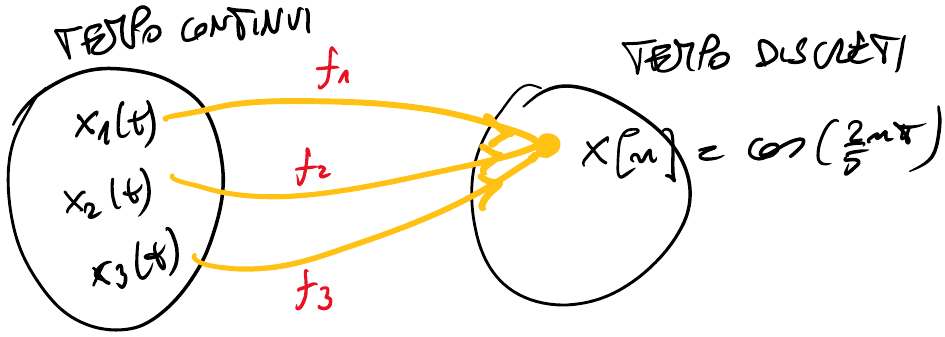
\includegraphics[scale=0.35]{immagini/lez9/stessoSegnale.jpg}
\end{figure}

\subsection{Ogni coseno discreto ha infiniti ALIAS SECONDARI, ma uno PRINCIPALE nell'intervallo}

Dato un segnale a tempo discreto, che chiamiamo ALIAS PRINCIPALE, posso costruire un altro segnale discreto identico ma con i termini diversi, che chiamiamo ALIAS SECONDARIO:

\[\begin{split}
    x_1[n] &= \cos(\frac{2}{5} \pi) = \cos(0,4 \pi n) \\
    x_2[n] &= \cos(0,4 \pi n + 2\pi n) = \cos(2,4 \pi n) =  \cos(0,4 \pi n) \\
    x_3[n] &= \cos(0,4 \pi n - 2\pi n) = \cos(-1,6 \pi n) =  \cos(1,6 \pi n) \\
\end{split}\]

Quindi ogni coseno discreto ha infiniti alias secondari, ma uno principale nell'intervallo $(-\pi]$, cioe' sappiamo quindi che la velocita' angolare $\Tilde{\omega}$ deve appartenere a questo intervallo. Espresso in termini di frequenza, sappiamo che la frequenza discreta $\Tilde{f} \in [-\frac{1}{2}, \frac{1}{2})$.

Nel mondo reale la frequenza puo' crescere all'infinito, mentre nel discreto non puo' mai superare $0,5$ altrimenti si ottiene un alias secondario del segnale originale.

\begin{table}[ht!]
    \centering
    \begin{tabular}{c|c|c|c|c}
         & $\cos(0,4 \pi n)$ & $\cos(2,4 \pi n)$ & $\cos(-0,4 \pi n)$ & $\cos(1,6 \pi n)$ \\
         \hline
        n=1 & 0,3090 & 0,3090 & 0,3090 & 0,3090 \\
        n=2 & -0,8090 & -0,8090 & -0,8090 & -0,8090 \\
        n=3 & -0,8090 & -0,8090 & -0,8090 & -0,8090 \\
        n=4 & 0,3090 & 0,3090 & 0,3090 & 0,3090 \\
        n=5 & 1,0000 & 1,0000 & 1,0000 & 1,0000 \\
    \end{tabular}
\end{table}

\subsubsection{Folded Alias}
Se trovo un'alias secondario che ha un segno negativo, posso spostare quel meno alla fase, ottenendo cosi' un Folded Alias, ovvero un alias con la fase cambiata di segno.

\[
    \cos(0,4 \pi n + \varphi) = \cos(\textcolor{red}{-}  1,6 \pi n + \varphi) = \cos(1,6 \pi n \textcolor{red}{-} \varphi)
\]

E se tolgo quel meno dalla fase trasformandolo in un complesso ottengo:
\[
    \cos(0,4 \pi n + \varphi + 2\pi h n) \rightarrow h \in \mathbf{Z}
\]

\section{Spettro}
Vediamo ora come ottenere lo spettro di un segnale tempo discreto.
Lo facciamo decomponendo il coseno con la formula di Eulero inversa:

\[
    x_1[n] = \cos(2\pi \Tilde{f} n + \varphi) = \frac{1}{2} e^{i \varphi} \cdot e^{i 2\pi \Tilde{f} n} + e^{-i \varphi} \cdot e^{-i 2\pi \Tilde{f} n}
\]

Il grafico del modulo dello spettro e':

\begin{figure}[ht!]
    \centering
    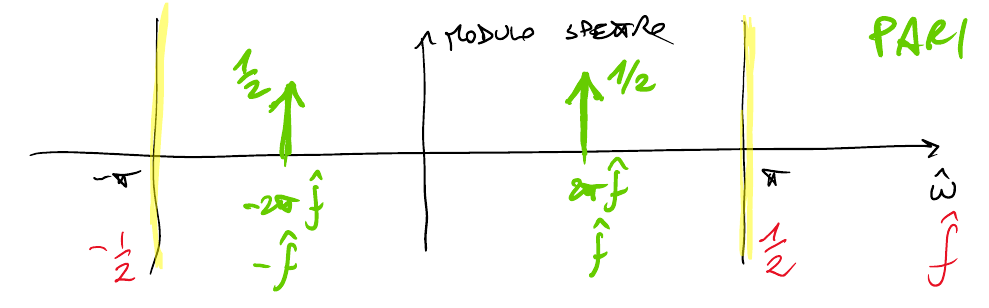
\includegraphics[scale=0.35]{immagini/lez10/spettroDiscreto.jpg}
\end{figure}

Ricordiamo che per essere formali, quando passiamo nel discreto disegno delle frecce e non solo barre, sia nel grafico del modulo che della fase.

Consideriamo ora un'altro segnale, che sappiamo essere un alias di quello precedente:

\[
    x_2[n] = \cos(2\pi \Tilde{f} n + \varphi + 2\pi n) = \frac{1}{2}e^{i \varphi} \cdot e^{i(2\pi \Tilde{f} + 2\pi)n} + \frac{1}{2}e^{-i \varphi} \cdot e^{-i(2\pi \Tilde{f} + 2\pi)n}
\]


Notiamo che nonostante i segnali siano degli alias hanno dei grafici diversi, questo perche' lo spettro di un segnale tempo discreto e' periodico, quindi contiene "righe" periodiche ($T = 2\pi$), che sono tutti gli spettri degli alias.

Questo ci fa intuire che l'unico segnale che posso ricostruire dato lo spettro e' l'alias principale (esempio frazioni).

\subsection{Esempio}
Abbiamo un segnale tempo continuo da campionare, provo varie frequenze di campionamento per vedere quale posso usare per ricostruire il segnale.

\[
    x(t) = \cos(2\pi \cdot 100t + \frac{\pi}{3})
\]

La prima frequenza di campionamento e' $f_s = 500$Hz:

\[
    x[n] = 2\cos(2\pi 100 \frac{n}{500} + \frac{\pi}{3}) = 2\cos(\frac{2\pi}{5} n + \frac{\pi}{3})
\]

Ora ricavo lo spettro:

\[
    x[n] = 1e^{i \frac{\pi}{3}} e^{i \frac{2}{5}\pi n} + 1e^{-i \frac{\pi}{3}} e^{-i \frac{2}{5}\pi n}
\]

Il grafico del modulo:

\begin{figure}[ht!]
    \centering
    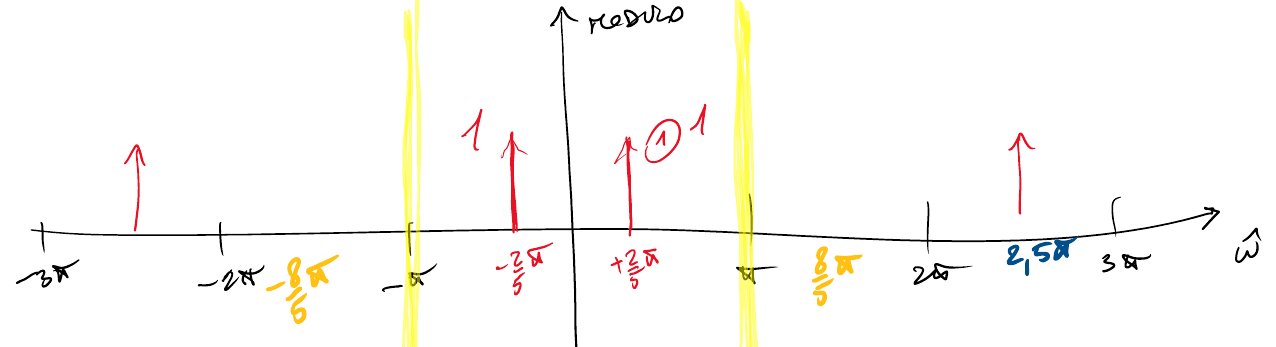
\includegraphics[scale=0.35]{immagini/lez10/moduloEsempio.jpg}
\end{figure}

Dal grafico noto che e' ottenuto l'alias principale, in quanto il modulo sta tra $-\pi, \pi$.
Quindi ricordando che $t = n \cdot T_c = \frac{n}{T_c}$ e che $n = t \cdot T_c$ posso ricostruire l'alias principale: 

\[
    x[t \cdot f_c] = 2\cos(\frac{2\pi}{5} \cdot t 500 + \frac{\pi}{3})
\]

Usiamo ora come frequenza di campionamento $f_s = 125$Hz:
\[
    x[n] = 2\cos(2\pi 100 \frac{n}{125}) = 2\cos(\frac{2\pi}{5} 4 n)
\]

tracciando il grafico:

\begin{figure}[ht!]
    \centering
    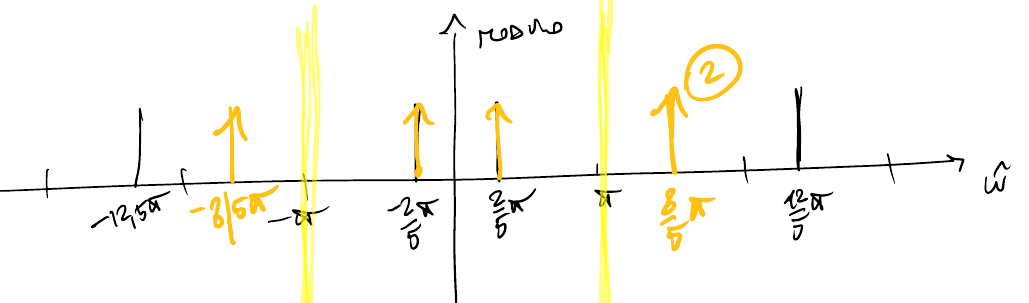
\includegraphics[scale=0.35]{immagini/lez10/moduloEsempio2.jpg}
\end{figure}
Noto che abbiamo ottenuto un'alias secondario, calcolo quindi quello principale:

\[
    x[n] = \cos(\frac{8}{5}\pi n + \frac{\pi}{3}) = \cos(\frac{8}{5} \pi n + \frac{\pi}{3} - 2\pi n) = \cos(-\frac{2}{5}\pi n + \frac{\pi}{3}) = \cos(\frac{2}{5} \pi n + \frac{\pi}{3})
\]

Posso quindi ricostruire solo l'alias principale (sostituendo ad n $t \cdot f_s$:

\[
    x[t \cdot f_s] = \cos(\frac{2}{5} \pi t 125 + \frac{\pi}{3})
\]

Usiamo ora come frequenza di campionamento $f_s = 100$Hz:

\[
    x[n] = 2\cos(2\pi 100 \frac{n}{100} + \frac{\pi}{3}) = 2\cos(2 \pi  n + \frac{\pi}{3})
\]

tracciando il grafico:

\begin{figure}[ht!]
    \centering
    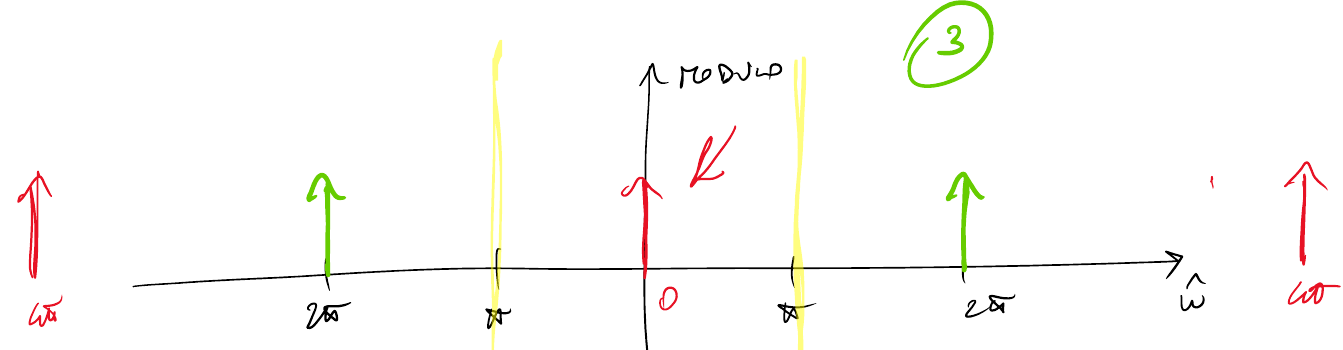
\includegraphics[scale=0.35]{immagini/lez10/moduloEsempio3.jpg}
\end{figure}
Noto che abbiamo ottenuto un'alias secondario, calcolo quindi quello principale:

\[
    x[n] = 2\cos(2\pi n + \frac{\pi}{3}) = 2\cos(\frac{\pi}{3}) \rightarrow x(t) = 2\cos(\frac{\pi}{3})
\]

Come ultimo esempio usiamo la frequenza di campionamento $f_s = 80$ Hz, da cui, come fatto fino ad ora, otteniamo il segnale campionato:

\[
    x[n] = 2\cos(2\pi 100 \frac{n}{80} + \frac{\pi}{3}) = 2\cos(2\pi \frac{5n}{4} + \frac{pi}{3})
\]

Tracciandone il grafico del modulo:

\begin{figure}[ht!]
    \centering
    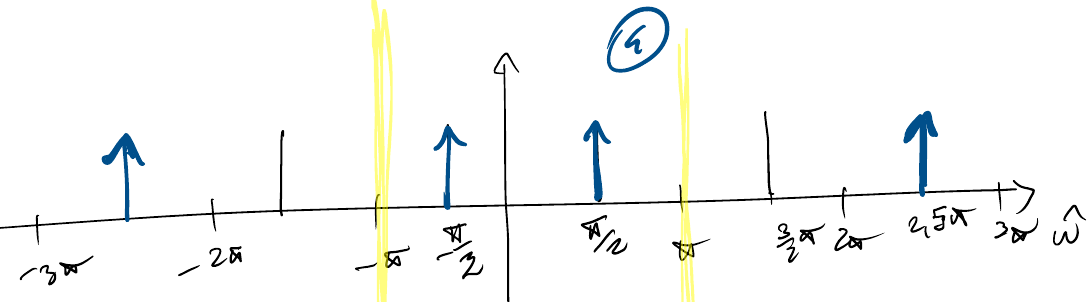
\includegraphics[scale=0.35]{immagini/lez10/moduloEsempio4.jpg}
\end{figure}

Notiamo ancora una volta che abbiamo ottenuto un alias secondario, quindi otteniamo quello principale e poi ricostruiamo il segnale:

\[
    x[n] = 2\cos(\frac{5}{2}\pi n + \frac{\pi}{3}) = 2\cos(\frac{\pi}{2} n + \frac{\pi}{3}) \rightarrow x(t) = 2\cos(\frac{\pi}{2} 80 t + \frac{\pi}{3}) = 2\cos(2\pi 20 t + \frac{\pi}{3})
\]

Le cose che dobbiamo ricordarci da questo esempio sono:

\begin{enumerate}
    \item Possiamo ricostruire solo un segnale che una volta campionato sta nell'alias principale (esistono infinite rappresentazioni dello spettro)
    \item Generalizzando l'esempio abbiamo potuto ricostruire il segnale solo se $\Tilde{omega}$ era nell'alias principale.
\end{enumerate}

Generalizziamo per capire in che intervallo dev'essere la velocita' angolare:

\[\begin{split}
    &\mbox{Segnale tempo continuo:}\\
    x(t) &= \cos(2\pi \cdot f_0 t) \rightarrow t = \frac{n}{f_s} \\
    &\mbox{Campionando otteniamo il segnale tempo discreto:} \\
    x[n] &= \cos(2\pi f_0 \cdot \frac{n}{f_s})\\
    2\pi \frac{f_0}{f_s} &= \Tilde{\omega} \rightarrow \mbox{Lo vogliamo nell'alias principale} \\
    -\pi &< 2\pi \frac{f_0}{f_s} \ne \pi \\
    f_s &> 2 |f_0| \\
\end{split}\]

Riassumendo vogliamo che la frequenza di campionamento $f_s$ sia il doppio del modulo di $f_0$ (frequenza cosinusoidale discreta) affinche' il segnale sia ricostruibile in modo esatto (Shannon).

\begin{figure}[ht!]
    \centering
    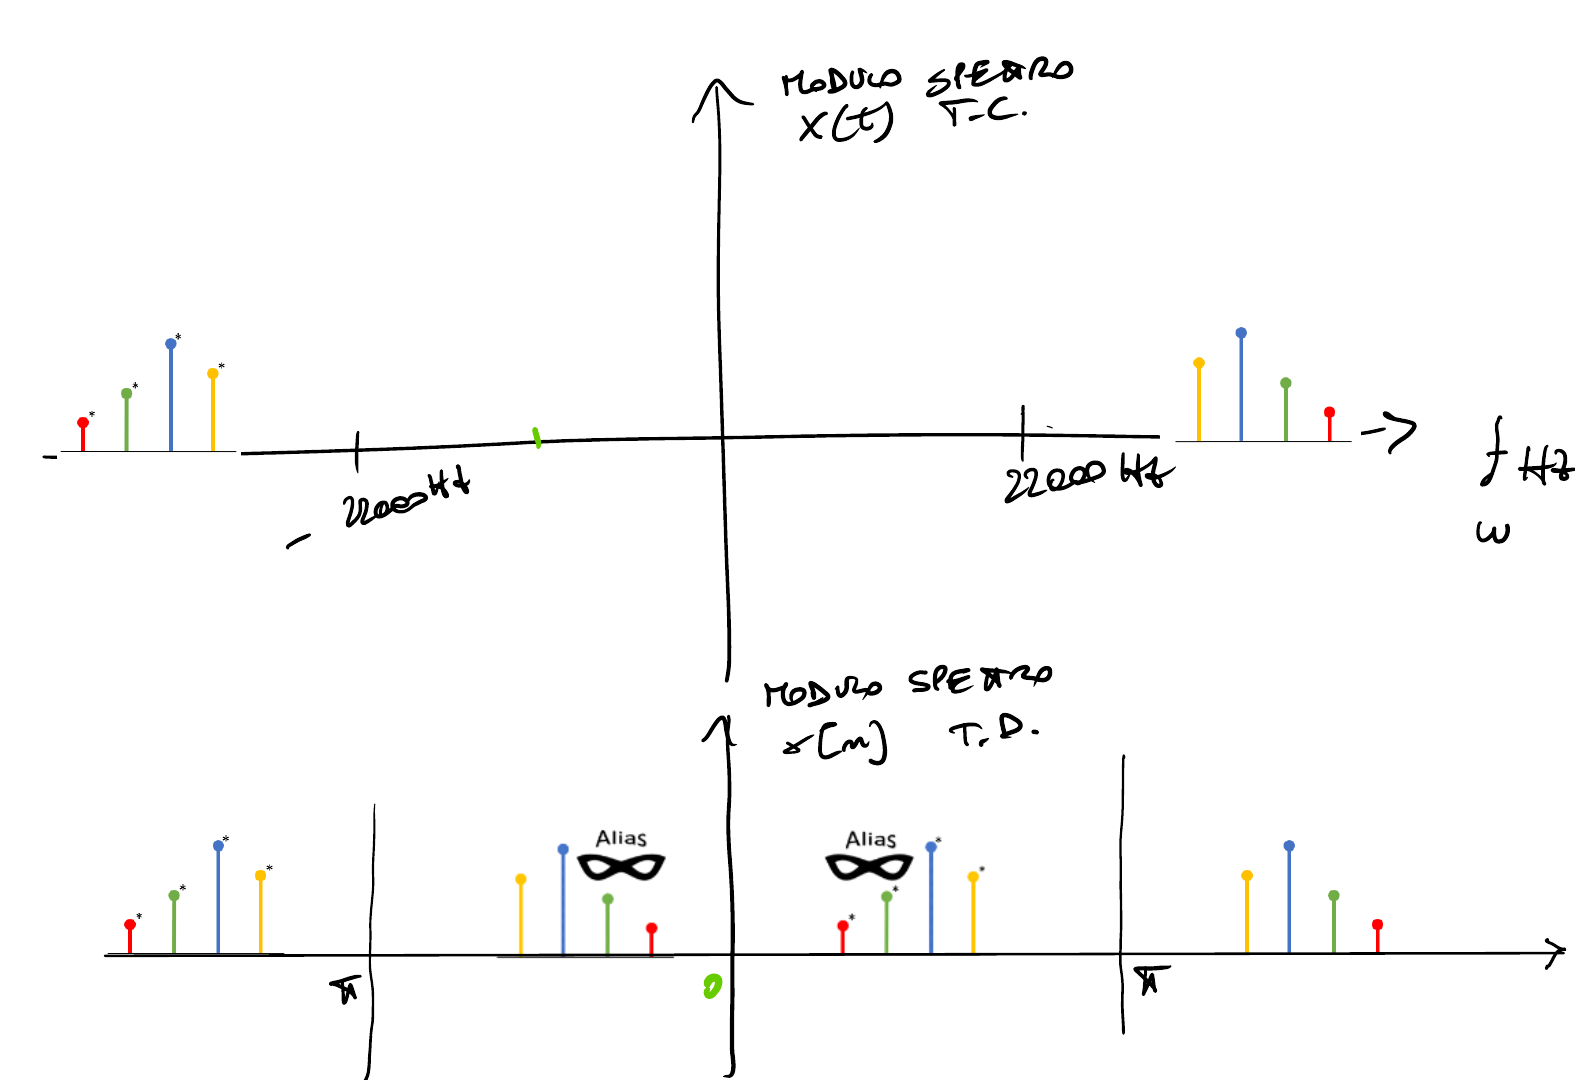
\includegraphics[scale=0.35]{immagini/lez11/spettroAlias.jpg}
\end{figure}

Quando campioniamo un segnale non rispettando il teorema di Shannon succede che le frequenze superano l'alias principale e di conseguenza vengono ribaltate creando rumore entrando nell'alias principale.

\section{Teorema del campionamento (Shannon)}
Dato un segnale tempo continui $x(t)$ a \textbf{banda limitata} B, lo si puo' ricostruire perfettamente dai propri campioni se e solo se

\[
    f_s = 2B
\]

Utilizzando un \underline{kernel di ricostruzione} ottimo

\[
    p(t)= \frac{\sin(\frac{\pi t}{T_s})}{\frac{\pi t}{T_s}} = sinc(\pi t f_s)
\]

Con banda limitata intendiamo un segnale composto da tante cosinusoidi ma che non vanno all'infinito, di conseguenza ne esiste una massima, quindi e' la frequenza massima appartenente ad un segnale. 

\begin{figure}[ht!]
    \centering
    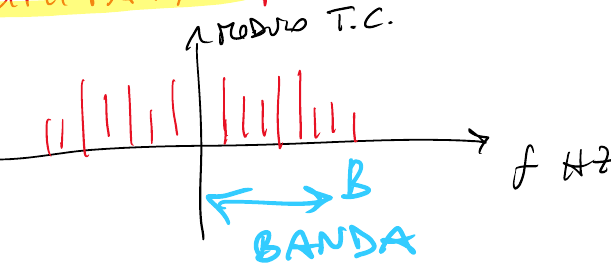
\includegraphics[scale=0.35]{immagini/lez10/banda.jpg}
\end{figure}

Diamo adesso della terminologia:
\begin{itemize}
    \item NYQUIST RATE: e' il doppio della frequenza massima $2B, 2F_{MAX}$. Noi dobbiamo sempre campionare usando una $f_s >$ della NYQUIST RATE.
    \item NYQUIST FREQUENCY: e' la meta' della frequenza di campionamento $\frac{f_s}{2}$.
\end{itemize}

\subsection{Ricostruire un segnale}
Ma effettivamente cosa vuol dire ricostruire un segnale? 
Se vogliamo capire la seconda parte del teorema di Shannon dobbiamo capire cosa si intende con kernel di ricostruzione.
Partiamo ripassando cosa significa interpolazione in linguaggio matematico. Significa trovare una funzione che passa da certi punti. Esistono molti modi di fare un'interpolazione, ad esempio lineare (colleghiamo linearmente due punti).
Nell'esempio in figura vediamo due tipi di interpolazione dati tre punti:

\begin{figure}[ht!]
    \centering
    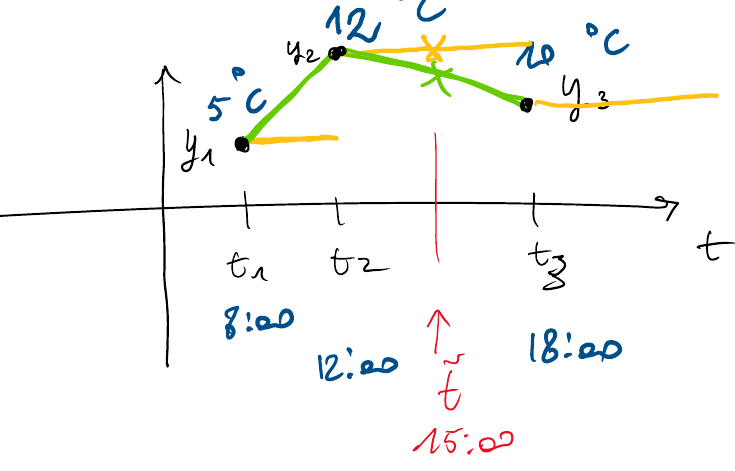
\includegraphics[scale=0.2]{immagini/lez10/interpolazione.jpg}
\end{figure}



Ricostruire un segnale e' come fare un interpolazione, abbiamo dei campioni e dobbiamo "collegare" i vari campioni per ricostruire un segnale quanto piu' possibile fedele all'originale.

Abbiamo vari modi di fare la ricostruzione, ad esempio esiste la ricostruzione di \underline{ordine zero (Z.0.H)}, in cui decido che il segnale negli intervalli e' costante. 
Il Kernel di ricostruzione in questo caso e' il rettangolo di altezza 1 in basso in figura, che e' come se prendessi e mettessi centrato per ogni campione e lo uso per ricostruire il segnale.

\begin{figure}[ht!]
    \centering
    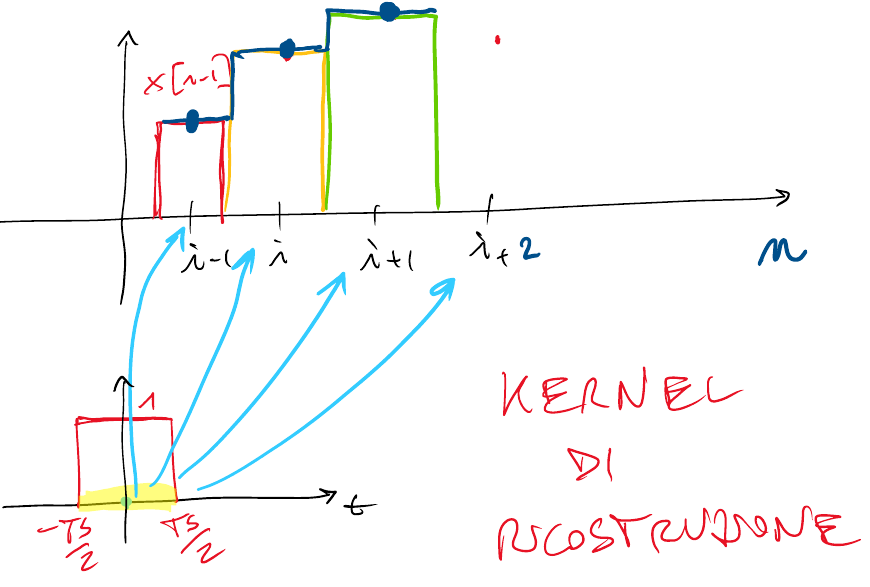
\includegraphics[scale=0.35]{immagini/lez10/ordineZero.jpg}
\end{figure}

Potremmo fare anche una ricostruzione lineare di primo grado, ovvero tracciamo una retta tra i vari campioni. In questo caso il kernel di ricostruzione e' un triangolo con base $-T, T$ ed alto 1, che prendiamo e posizioniamo su ogni campione, e sommiamo tutti i triangoli. Ovviamente come si nota dal grafico ci sono delle sovrapposizioni tra i trinagoli:

\begin{figure}[ht!]
    \centering
    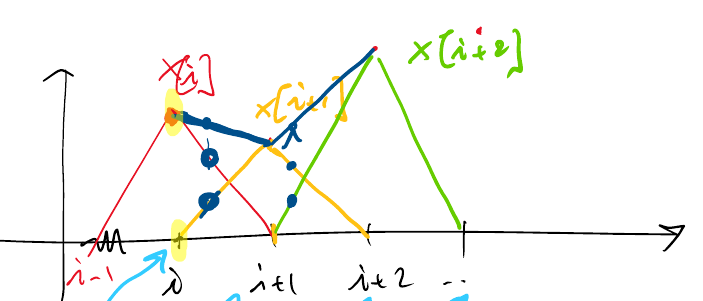
\includegraphics[scale=0.35]{immagini/lez10/lineare.jpg}
\end{figure}

\medskip
\medskip
\medskip
\medskip
\medskip
\medskip
\medskip
\medskip
\medskip
\medskip
\medskip
\medskip
\medskip
\medskip
\medskip
\medskip
\medskip
\medskip


\subsubsection{Dimostrazione ricostruzione lineare}
Dimostriamo che effettivamente la ricostruzione lineare funziona.
Inizialmente abbiamo un grafico in cui sono presenti due punti:

\begin{figure}[ht!]
    \centering
    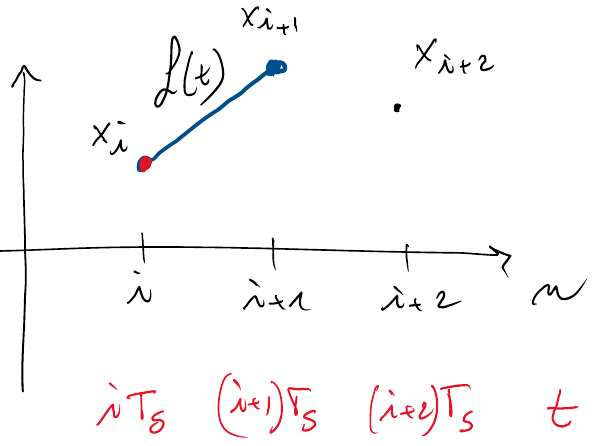
\includegraphics[scale=0.35]{immagini/lez10/linearePartenza.jpg}
\end{figure}

noi dato che stiamo ricostruendo linearmente dobbiamo tracciare una linea retta tra i due punti, e quello che otteniamo la chiamiamo $f(t)$, che e' l'equazione della retta che passa dai due punti:

\[
    f(t) = (t-i T_s) \frac{x_{i+1} - x_i}{(i + 1)T_s - i T_s} + x_i
\]

Facciamo due verifiche per capire che l'equazione e' corretta:

\[\begin{split}
    f(i T_s) &= (i T_s - i T_s) \frac{x_{i+1} - x_i}{(i+1)T_s - i T_s} + x_1 = x_i \\
    f((i + 1)T_s) &= ((i+1)T_s - i T_s) \frac{x_{i+1} - x_i}{(i + 1) T_s - i T_s} + x_i = x_{i+1}
\end{split}\]

Verificato che l'equazione passa effettivamente per quei punti, portiamo tutti i termini (dell'equazione della retta) che dipendono da $x_i$ a sinistra e tutti quelli che dipendono da $x_{i+1}$ a destra:

\[
    x(t) = -\frac{x_i}{T_s} (t - i T_s) + x_i +\frac{x_{i+1}}{T_s} (t - i T_s)
\]

E notiamo che la parte sinistra dell'equazione e' la retta che parte dal punto $x_i$ ed arriva a $i+1$, mentre la parte di destra e' la retta che parte da $x_{i+1}$ ed arriva ad $i$. Quindi la retta che passa tra i due punti e' la somma dei segmenti ottenuti precedentemente. 
E se ripetiamo questo procedimento utilizzando la parte sinistra per il punto $x_{i+1}$ e la parte destra per il punto $x_i$, notiamo che si ottiene un triangolo, che e' il kernel di ricostruzione.

\begin{figure}[ht!]
    \centering
    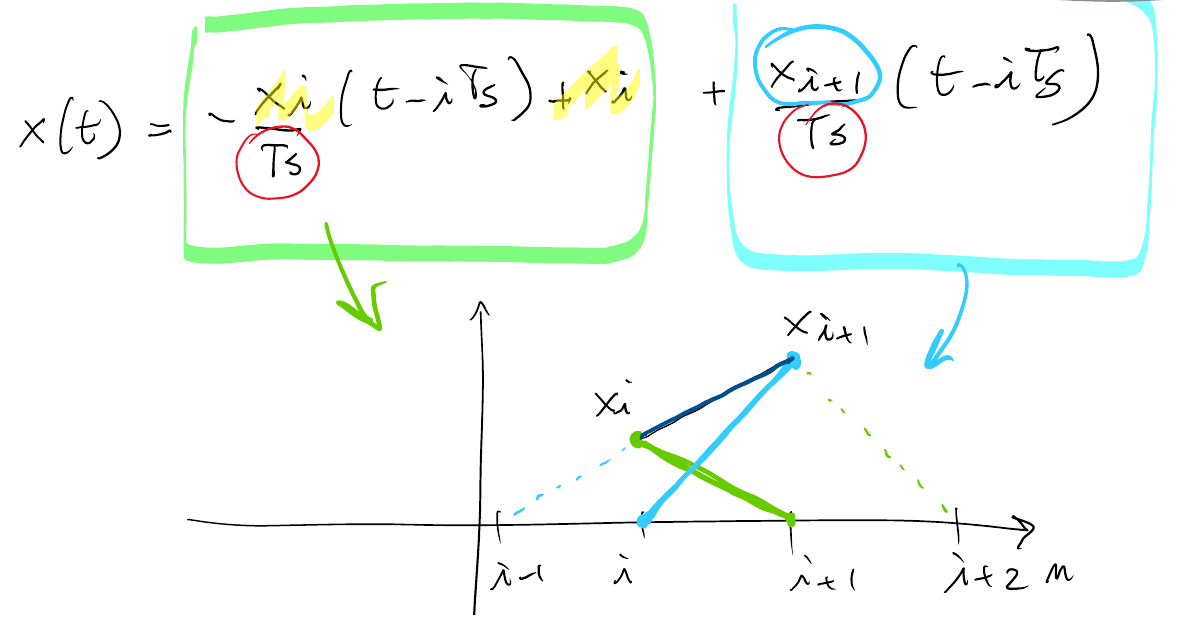
\includegraphics[scale=0.35]{immagini/lez10/lineareDimostrazione.jpg}
\end{figure}

\subsection{Funzionamento kernel ottimo}
Il kernel di interpolazione ottimo previsto da Shannon ricordiamo essere:

\[\begin{split}
     P(t)=
    \begin{cases}
    \frac{\sin \pi t F_s}{\pi t F_s} \text{ se } t \ne 0 \\
    1 \text{ se } t = 0 \\
    \end{cases}
    = sinc \pi t F_s
\end{split}
\]

\begin{figure}[ht!]
    \centering
    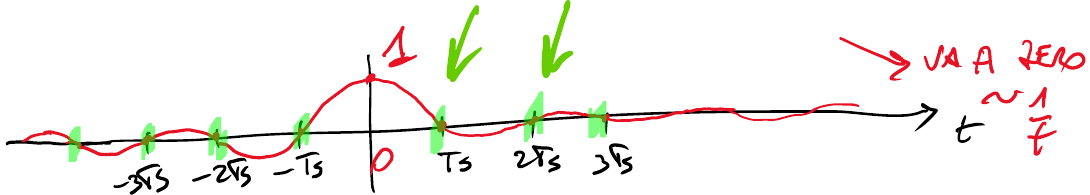
\includegraphics[scale=0.35]{immagini/lez12/kernelOttimo.jpg}
\end{figure}

Ma come funziona? E' una funzione che oscilla da meno a piu' infinito, pari e si rastrema all'infinito come $\frac{1}{T}$, come un iperbole, che va a zero lentamente. Inoltre passa per zero tutte le volte che $\pi t f_s = k \pi, k \in \mathbf{Z}$, ovvero $t = \frac{1}{f_s} k = k \cdot T_s$.
E' zero in tutti i campioni (dove passa la griglia di campionamento) eccetto lo zero, dove vale 1.
Quello che dobbiamo fare e' prendere questo kernel e giustapporrlo ad ogni campione e poi sommarli.

Esempio:

\begin{figure}[ht!]
    \centering
    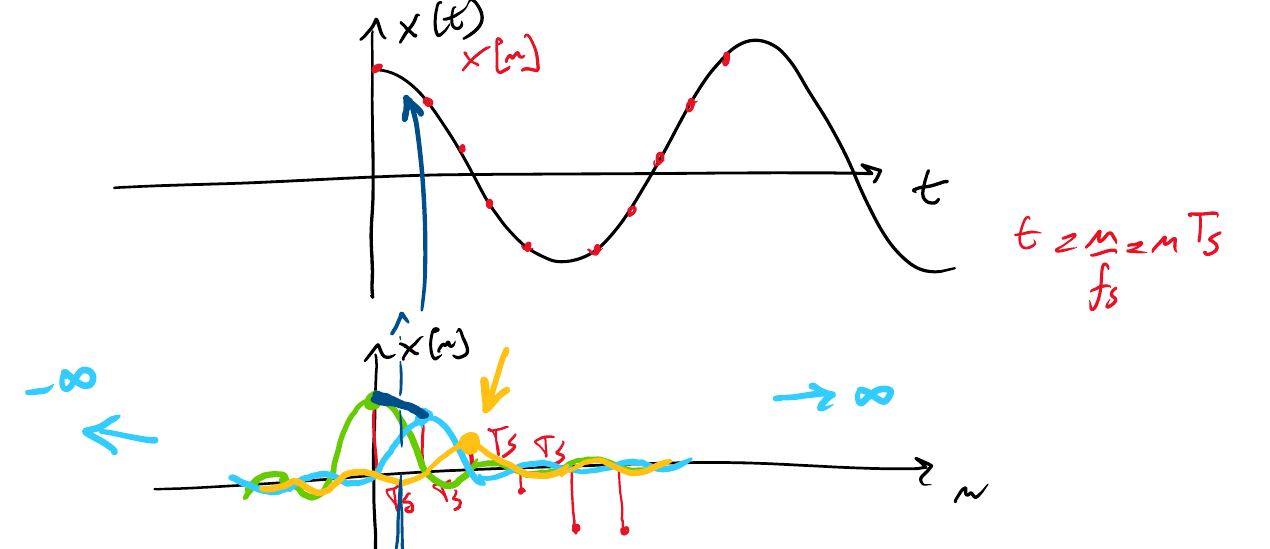
\includegraphics[scale=0.35]{immagini/lez12/usoKernelOttimo.jpg}
\end{figure}

dobbiamo prendere il kernel di ricostruzione e modularlo su ogni punto, non possiamo fermarci da $-T_s, T_s$ ma va fatto per tutti i campioni, fino ad infinito.

Ma dato che nella realta' abbiamo un numero di campioni finito lo possiamo usare.
Ora ipotizzando una canzone di 4 minuti ed ipotizzando di campionarla a 44100 campioni al secondo (che e' quello che si fa nella realta'), per ricostruire perfettamente il segnale dovremmo avere 10584000 kernel. Quindi capiamo che per un problema di prestazioni raramente si usa questo kernel per ricostruire i segnali, ma ci accontentiamo del fatto che un segnale rispetti il teorema di Shannon e poi usiamo un kernel piu' facile (ad esempio lineare, 0, quadratico).